\documentclass[cn,chinese,color=cyan]{elegantbook}
%\definecolor{second}{RGB}{244, 105, 102}
\title{Python全栈开发(中级)}
\subtitle{课程学习记录}

\author{雨霓同学}
\institute{鸢}
\date{2020年6月19日}
\version{910014191@qq.com}
\bioinfo{版本}{V1.0}


\extrainfo{没有合格的黑夜,也就无所谓真正的黎明}
\setcounter{tocdepth}{3}

\newcommand{\dollar}{\mbox{\textdollar}}
\lstset{
	mathescape = false}
\logo{logo1.png}
\cover{(2).jpg}

% 本文档命令
\usepackage{mathtools}
\usepackage{background}
\usepackage{varwidth}
\usepackage{tikz} 
\SetBgContents{}
\usepackage{array}
\usepackage{halloweenmath}
\usepackage{float}
\usepackage{algorithm}  
\usepackage{algpseudocode}  
\usepackage{float}
\usepackage{longtable}
\usepackage{multirow}
\usepackage{booktabs}
\usepackage{varwidth}
\usepackage{natbib}
\usepackage{multirow}
\usepackage{booktabs}
\usepackage[many]{tcolorbox}
\tcbuselibrary{skins, breakable, theorems}
\tcbuselibrary{listings}
\tcbuselibrary{breakable}
\tcbset{boxrule=0pt,sharp corners}
\tcbset{listing options=Python}

\lstdefinestyle{Python2}{
	language =   Python, % 语言选Python
	frame=none,
	mathescape,
	emphstyle={\color{frenchplum}},
	numbers=none,
	stepnumber=2,
	numbersep=3em,
	numberstyle=\tiny,
	keywordstyle    =   \color{blue},
	keywordstyle    =   [2] \color{teal},
	stringstyle     =   \color{magenta},
	commentstyle    =   \color{red}\ttfamily,
	breaklines      =   true,   % 自动换行,
	columns         =   fixed,  %字间距就不固定很丑,必须加
	basewidth       =   .5em,
	keywordstyle=\color{red},
	commentstyle=\color{gray},
	backgroundcolor=\color[RGB]{252, 252, 252},
	tabsize=4,
	showspaces=false,
	showstringspaces=false,
	columns=fixed,
	morekeywords={maketitle,pip,matplotlib,pandas,numpy},
}

\newtcolorbox{notes}[1][]{%
	enhanced jigsaw,
	borderline west={1.5pt}{0pt}{mblue},
	sharp corners,
	boxrule=0pt,
	fonttitle={\small\bfseries},
	coltitle={black},
	title={{\color{mblue} \faInfoCircle} Note:\ },
	colbacktitle=mlblue,
	colback=bg,
	left=2mm,
	right=2mm,
	#1}
\newtcolorbox{code}[1][]{%
	enhanced jigsaw,
	breakable,
	borderline west={1.5pt}{0pt}{mblue},
	sharp corners,
	boxrule=0pt,
	fonttitle={\small\bfseries},
	coltitle={black},
	title={{\color{mblue} \faCode} \quad Python Code:\ },
	colbacktitle=mlblue,
	colback=bg,
	left=2mm,
	right=2mm,
	#1}
\newtcolorbox{warning}[1][]{%
	enhanced jigsaw,
	breakable,
	borderline west={1.5pt}{0pt}{mred},
	sharp corners,
	boxrule=0pt,
	fonttitle={\small\bfseries},
	coltitle={black},
	title={{\color{mred} \faExclamationTriangle} Warning:\ },
	colbacktitle=mlred,
	colback=bg,
	left=2mm,
	right=2mm,
	#1}

\usepackage{varwidth}
 
\newlist{tabitemize}{itemize}{1}
\setlist[tabitemize]{label=\ding{118},nosep,after=\strut}












\numberwithin{equation}{section}
\usepackage{cases,empheq}
\usepackage{tabularx}
\usepackage[T1]{fontenc}
\usepackage{xcolor}
\definecolor{bg}{rgb}{0.99,0.99,0.99}
\definecolor{mlblue}{RGB}{236,243,255}
\definecolor{mblue}{RGB}{0,123,255}
\definecolor{mlred}{RGB}{253,243,242}
\definecolor{mred}{RGB}{220,53,69}
\usepackage{newtxtext}
\usepackage[UTF8,scheme=plain]{ctex}
\usepackage{fontawesome}
\usepackage{newtxtext}

\definecolor{pblue}{rgb}{0.13,0.13,1}
\definecolor{pgreen}{rgb}{0,0.5,0}
\definecolor{darkblue}{cmyk}{1,0,0,0}%纯蓝
\renewcommand{\headrule}{\color{darkblue}\leavevmode\xleaders\hbox{${\sim}{\cdot}$}\hfill\null}

\pagestyle{fancy}
\newcommand{\ccr}[1]{\makecell{{\color{#1}\rule{1cm}{1cm}}}}
% 修改目录深度
\setcounter{tocdepth}{2}

\begin{document}
\definecolor{mycolor}{RGB}{245, 255, 250}%用于设置封面长条颜色
\maketitle



\frontmatter



%但是,我想声明的是:

%\begin{center}
%  由于某些原因,Elegant\LaTeX{} 项目 \underline{不再接受}\textbf{任何}非我本人预约的提交。
%\end{center}

%我是一个理想主义者,关于这个模板,我有自己的想法。我所关心的是,我周围的人能方便使用 \LaTeX{} 以及此模板,我自己会为自己的东西感到开心。如果维护模板让我不开心,那我就不会再维护了。诚然这个模板并不是完美的,但是相比 2.x 好很多了,这些改进离不开大家的反馈、China\TeX{} 和逐鹿人的鼓励以及支援人员的帮助!

%\vskip 1.5cm

%\begin{flushright}
%Ethan Deng\\
%February 10, 2020
%\end{flushright}
\newpage 
\tableofcontents
%\listofchanges

\mainmatter
\chapter{网络编程——SOCKET开发}
\section{计算机基础}
\subsection{什么是C/S架构}
C指的是client(客户端软件),S指的是Server(服务端软件),本章的重点就是教大家写一个C/S架构的软件,实现服务端软件与客户端软件基于网络通信。


作为应用开发程序员,我们开发的软件都是应用软件,而应用软件必须运行于操作系统之上,操作系统则运行于硬件之上,应用软件是无法直接操作硬件的,应用软件对硬件的操作必须调用操作系统的接口,由操作系统操控硬件。

比如客户端软件想要基于网络发送一条消息给服务端软件,流程是:

\begin{dinglist}{118}
	\item 客户端软件产生数据,存放于客户端软件的内存中,然后调用接口将自己内存中的数据发送/拷贝给操作系统内存
	
	\item 客户端操作系统收到数据后,按照客户端软件指定的规则(即协议)、调用网卡发送数据
	
	\item 网络传输数据
	
	\item 服务端软件调用系统接口,想要将数据从操作系统内存拷贝到自己的内存中
	
	\item 服务端操作系统收到4的指令后,使用与客户端相同的规则(即协议)从网卡接收到数据,然后拷贝给服务端软件
\end{dinglist}

\subsection{什么是网络}

硬件之上安装好操作系统,然后装上软件你就可以正常使用了,但此时你也只能自己使用,像下图这样,每个人都拥有一台自己的机器,然而彼此孤立



如何能大家一起玩耍,那就是联网了,即internet



然而internet为何物?举一个简单的例子: 如果把一个人与这个人的有线电话比喻为一台计算机,那么其实两台计算机之间通信与两个人打电话之间通信的原理是一样的。 两个人之间想要打电话首先一点必须是接电话线,这就好比是计算机之间的通信首先要有物理链接介质,比如网线,交换机,路由器等网络设备。 通信的线路建好之后,只是物理层面有了可以承载数据的介质,要想通信,还需要我们按照某种规则组织我们的数据,这样对方在接收到数据后就可以按照相同的规则去解析出数据,这里说的规则指的就是:中国有很多地区,不同的地区有不同的方言,为了全中国人都可以听懂,大家统一讲普通话



普通话属于中国国内人与人之间通信的标准,那如果是两个国家的人交流呢?



问题是,你不可能要求一个人/计算机掌握全世界的语言/标准,于是有了世界统一的通信标准:英语



英语成为世界上所有人通信的统一标准,计算机之间的通信也应该有一个像英语一样的通信标准,这个标准称之为互联网协议, 可以很明确地说:互联网协议就是计算机界的英语,网络就是物理链接介质+互联网协议。 我们需要做的是,让全世界的计算机都学会互联网协议,这样任意一台计算机在发消息时都严格按照协议规定的格式去组织数据,接收方就可以按照相同的协议解析出结果了,这就实现了全世界的计算机都能无障碍通信。

 按照功能不同,人们将互联网协议分为osi七层或tcp/ip五层或tcp/ip四层(我们只需要掌握tcp/ip五层协议即可),这种分层就好比是学习英语的几个阶段,每个阶段应该掌握专门的技能或者说完成特定的任务,比如:1、学音标 2、学单词 3、学语法 4、写作文。。。



每层运行常见物理设备(了解)

\subsection{什么是TCP/IP?}
Transmission Control Protocol/Internet Protocol的简写,中译名为传输控制协议/因特网互联协议,又名网络通讯协议,是Internet最基本的协议、Internet国际互联网络的基础

\subsection{TCP/IP的起源}
20世纪50年代末,正处于冷战时期。当时美国军方为了自己的计算机网络在受到袭击时,即使部分网络被摧毁,其余部分仍能保持通信联系,便由美国国防部的高级研究计划局(ARPA)建设了一个军用网,叫做“阿帕网”(ARPAnet)。阿帕网于1969年正式启用,当时仅连接了4台计算机,供科学家们进行计算机联网实验用,这就是因特网的前身。

到70年代,ARPAnet已经有了好几十个计算机网络,但是每个网络只能在网络内部的计算机之间互联通信,不同计算机网络之间仍然不能互通。为此, ARPA又设立了新的研究项目,支持学术界和工业界进行有关的研究,研究的主要内容就是想用一种新的方法将不同的计算机局域网互联,形成“互联网”。研究人员称之为“internetwork”,简称“Internet”,这个名词就一直沿用到现在。

终于到1974年,TCP/IP诞生啦,TCP/IP有一个非常重要的特点,就是开放性,即TCP/IP的规范和Internet的技术都是公开的。目的就是使任何厂家生产的计算机都能相互通信,使Internet成为一个开放的系统,这正是后来Internet得到飞速发展的重要原因。

\subsection{OSI七层模型}

美国国防部在开发tcp/ip的同时,还有一些其它大厂商也开发出了自己的网络体系,实际上世界上第一个网络体系结构由IBM公司提出(也是74年,比TCP/IP略早,SNA),以后其他公司也相继提出自己的网络体系结构如:Digital公司的DNA,美国国防部的TCP/IP等,多种网络体系结构并存,其结果是若采用IBM的结构,只能选用IBM的产品,只能与同种结构的网络互联。

这就像中国人说中文,美国人说英语,日本人说日本话一样,同一国家的人沟通没问题,但不同国家之间的人没法通信。为了解决网络通信中这样不互通的问题,国际标准化组织ISO于1977年成立了一个委员会,在现有网络的基础上,提出了不基于具体机型、操作系统或公司的网络体系结构,称为开放系统互联模型。

\chapter{混沌与混乱}
\section{IP、MAC和端口号}

\subsection{IP地址}

IP地址是 Internet Protocol Address 的缩写,译为“网际协议地址”。

目前大部分软件使用 IPv4 地址,但 IPv6 也正在被人们接受,尤其是在教育网中,已经大量使用。

一台计算机可以拥有一个独立的 IP 地址,一个局域网也可以拥有一个独立的 IP 地址(对外就好像只有一台计算机)。对于目前广泛使用 IPv4 地址,它的资源是非常有限的,一台计算机一个 IP 地址是不现实的,往往是一个局域网才拥有一个 IP 地址。

在因特网上进行通信时,必须要知道对方的 IP 地址。实际上数据包中已经附带了 IP 地址,把数据包发送给路由器以后,路由器会根据 IP 地址找到对方的地里位置,完成一次数据的传递。路由器有非常高效和智能的算法,很快就会找到目标计算机。


\subsection{MAC地址}
现实的情况是,一个局域网往往才能拥有一个独立的 IP;换句话说,IP 地址只能定位到一个局域网,无法定位到具体的一台计算机。这可怎么办呀?这样也没法通信啊。

其实,真正能唯一标识一台计算机的是 MAC 地址,每个网卡的 MAC 地址在全世界都是独一无二的。计算机出厂时,MAC 地址已经被写死到网卡里面了(当然通过某些“奇巧淫技”也是可以修改的)。局域网中的路由器/交换机会记录每台计算机的 MAC 地址。


MAC 地址是 Media Access Control Address 的缩写,直译为“媒体访问控制地址”,也称为局域网地址(LAN Address),以太网地址(Ethernet Address)或物理地址(Physical Address)。
数据包中除了会附带对方的 IP 地址,还会附带对方的 MAC 地址,当数据包达到局域网以后,路由器/交换机会根据数据包中的 MAC 地址找到对应的计算机,然后把数据包转交给它,这样就完成了数据的传递。

\subsection{端口号}
有了 IP 地址和 MAC 地址,虽然可以找到目标计算机,但仍然不能进行通信。一台计算机可以同时提供多种网络服务,例如 Web 服务(网站)、FTP 服务(文件传输服务)、SMTP 服务(邮箱服务)等,仅有 IP 地址和 MAC 地址,计算机虽然可以正确接收到数据包,但是却不知道要将数据包交给哪个网络程序来处理,所以通信失败。

为了区分不同的网络程序,计算机会为每个网络程序分配一个独一无二的端口号(Port Number),例如,Web 服务的端口号是 80,FTP 服务的端口号是 21,SMTP 服务的端口号是 25。

端口(Port)是一个虚拟的、逻辑上的概念。可以将端口理解为一道门,数据通过这道门流入流出,每道门有不同的编号,就是端口号。


\section{TCP基本认识}
我们先来看看 TCP 头的格式,标注颜色的表示与本文关联比较大的字段,其他字段不做详细阐述。
\begin{figure}[H]
	\centering
	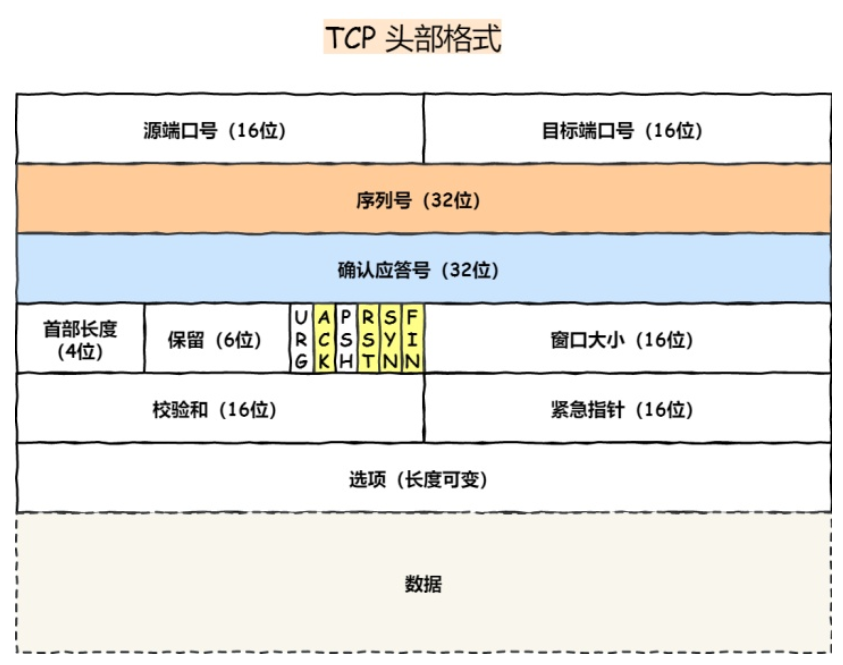
\includegraphics[width=\linewidth]{a1.png}
\end{figure}

\begin{dinglist}{118}
	

\item \textbf{序列号:}在建立连接时由计算机生成的随机数作为其初始值,通过 SYN 包传给接收端主机,每发送一次数据,就「累加」一次该「数据字节数」的大小。\textbf{用来解决网络包乱序问题。}


\item \textbf{确认应答号:}指下一次「期望」收到的数据的序列号,发送端收到这个确认应答以后可以认为在这个序号以前的数据都已经被正常接收\textbf{。用来解决不丢包的问题。}


\item  \textbf{控制位:}

\begin{enumerate}
	\item ACK:该位为 1 时,「确认应答」的字段变为有效,TCP 规定除了最初建立连接时的 SYN 包之外该位必须设置为 1 。
	
	\item RST:该位为 1 时,表示 TCP 连接中出现异常必须强制断开连接。
	
\item 	SYN:该位为 1 时,表示希望建立连,并在其「序列号」的字段进行序列号初始值的设定。
	
	\item FIN:该位为 1 时,表示今后不会再有数据发送,希望断开连接。当通信结束希望断开连接时,通信双方的主机之间就可以相互交换 FIN 位置为 1 的 TCP 段。
\end{enumerate}
\end{dinglist}

\subsection{为什么需要TCP协议?TCP工作在哪一层}
IP 层是「不可靠」的,它不保证\textbf{网络包的交付}、\textbf{不保证网络包的按序交付}、\textbf{也不保证网络包中的数据的完整性}。如果需要保障网络数据包的可靠性,那么就需要由上层(传输层)的 TCP 协议来负责。

因为 TCP 是一个工作在\textbf{传输层}的\textbf{可靠}数据传输的服务,它能确保接收端接收的网络包是\textbf{无损坏、无间隔、非冗余和按序的}。

\subsection{什么是TCP?}
\begin{dinglist}{118}
	\item \textbf{面向连接:}一定是「一对一」才能连接,不能像 UDP 协议 可以一个主机同时向多个主机发送消息,也就是一对多是无法做到的;
	
	\item \textbf{可靠的:}无论的网络链路中出现了怎样的链路变化,TCP 都可以保证一个报文一定能够到达接收端;
	
	\item \textbf{字节流:}消息是「没有边界」的,所以无论我们消息有多大都可以进行传输。并且消息是「有序的」,当「前一个」消息没有收到的时候,即使它先收到了后面的字节已经收到,那么也不能扔给应用层去处理,同时对「重复」的报文会自动丢弃。

\end{dinglist}

简单来说就是,\textbf{用于保证可靠性和流量控制维护的某些状态信息,这些信息的组合,包括Socket、序列号和窗口大小称为连接。}

\textbf{Socket:}由 IP 地址和端口号组成

\textbf{序列号:}用来解决乱序问题等

\textbf{窗口大小:}用来做流量控制

\subsection{什么是socket?}
为了区分应用程序(进程)之间的网络通信和连接,需要传输层协议(TCP、UDP),目的IP地址和端口号这三个参数进行标识,将这三个参数结合起来,就成为套接字,又称插座。

应用层可以与传输层通过套接字接口区分来自不同应用程序或网络连接的通信,套接字代表TCP/IP网络中唯一 的网络进程,通过源主机的一个套接字与目标主机的一个套接字,就可以在两个主机之间建立一个连接。

\subsection{如何唯一确定一个 TCP 连接呢?}
TCP 四元组可以唯一的确定一个连接,四元组包括如下:
\begin{dinglist}{118}
	\item \textbf{源地址:} 源地址和目的地址的字段(32位)是在 IP 头部中,作用是通过 IP 协议发送报文给对方主机。
	\item \textbf{源端口 } 源端口和目的端口的字段(16位)是在 TCP 头部中,作用是告诉 TCP 协议应该把报文发给哪个进程。
	\item 目的地址
\item 	目的端口
\end{dinglist}

\subsection{UDP和TCP有什么区别呢?}
UDP 不提供复杂的控制机制,利用 IP 提供面向「无连接」的通信服务。

UDP 协议真的非常简,头部只有 8 个字节( 64 位),UDP 的头部格式如下:

\begin{figure}[H]
	\centering
	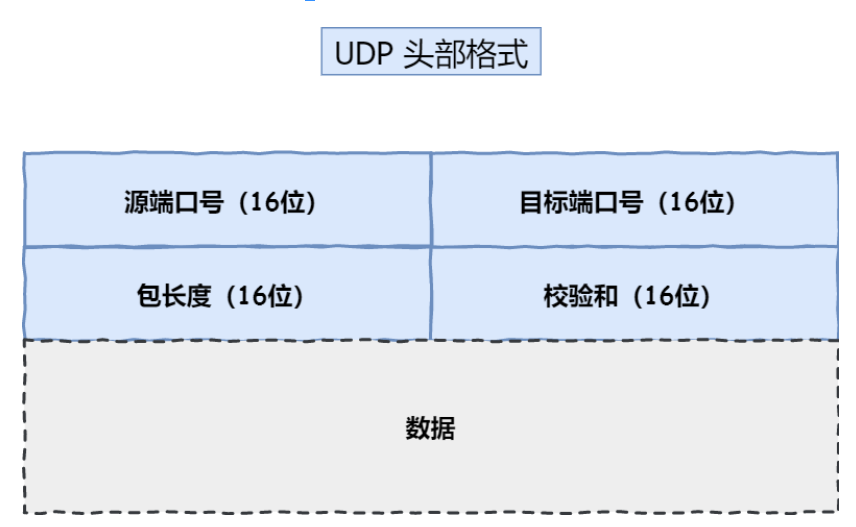
\includegraphics[width=\linewidth]{a2.png}
\end{figure}
\begin{dinglist}{118}
	\item 目标和源端口:主要是告诉 UDP 协议应该把报文发给哪个进程。
	\item 包长度:该字段保存了 UDP 首部的长度跟数据的长度之和。
	\item 校验和:校验和是为了提供可靠的 UDP 首部和数据而设计
\end{dinglist}
\subsection{TCP与UDP区别和应用场景}
\begin{enumerate}
	\item \textbf{连接}
	
	TCP 是面向连接的传输层协议,传输数据前先要建立连接。
	
	UDP 是不需要连接,即刻传输数据。
	
	\item \textbf{服务对象}
	
	TCP 是一对一的两点服务,即一条连接只有两个端点。
	
	UDP 支持一对一、一对多、多对多的交互通信
	
	\item \textbf{ 可靠性}
	
	TCP 是可靠交付数据的,数据可以无差错、不丢失、不重复、按需到达。
	
	UDP 是尽最大努力交付,不保证可靠交付数据。
	
	\item \textbf{拥塞控制、流量控制}
	
	TCP有拥塞控制和流量控制机制,保证数据传输的安全性。
	
	UDP 则没有,即使网络非常拥堵了,也不会影响 UDP 的发送速率。
	
	\item\textbf{ 首部开销}
	
	TCP 首部长度较长,会有一定的开销,首部在没有使用「选项」字段时是 20 个字节,如果使用了「选项」字段则会变长的。
	
	UDP 首部只有 8 个字节,并且是固定不变的,开销较小。
\end{enumerate}

\textbf{TCP 和 UDP 应用场景:}

\begin{dinglist}{118}
	\item 由于 TCP 是面向连接,能保证数据的可靠性交付,因此经常用于:
	
	FTP 文件传输
	
	HTTP / HTTPS
	
	\item 由于 UDP 面向无连接,它可以随时发送数据,再加上UDP本身的处理既简单又高效,因此经常用于:
	
	包总量较少的通信,如 DNS 、SNMP 等
	
	视频、音频等多媒体通信广播通信
\end{dinglist}

\section{TCP 连接建立}
\subsection{TCP三次握手过程和状态变迁}
TCP 是面向连接的协议,所以使用 TCP 前必须先建立连接,而建立连接是通过三次握手而进行的。
\begin{figure}[H]
	\centering
	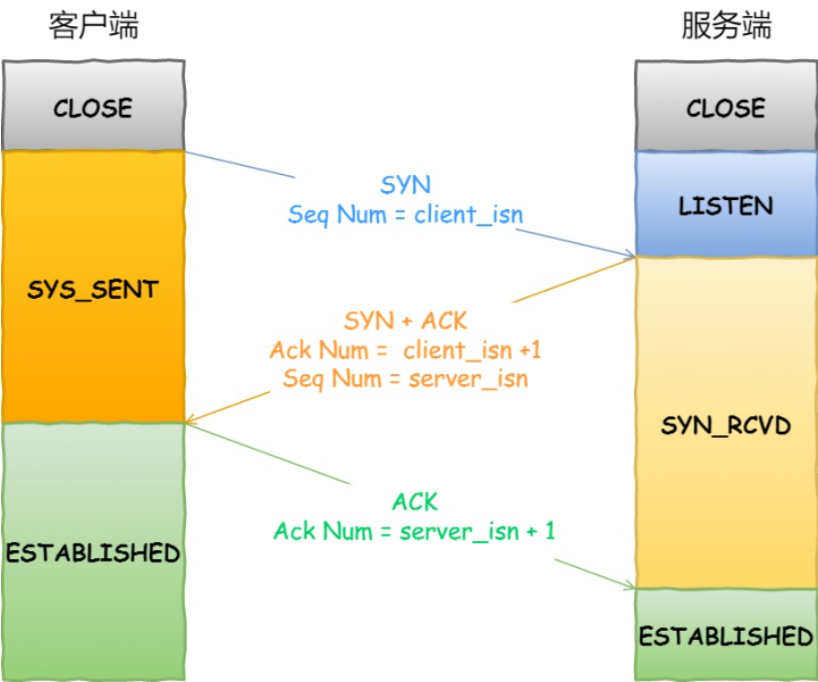
\includegraphics[width=.6\linewidth]{a3.png}
\end{figure}
\begin{dinglist}{118}
	\item 一开始,客户端和服务端都处于 CLOSED 状态。先是服务端主动监听某个端口,处于 LISTEN状态
	\begin{figure}[H]
		\centering
		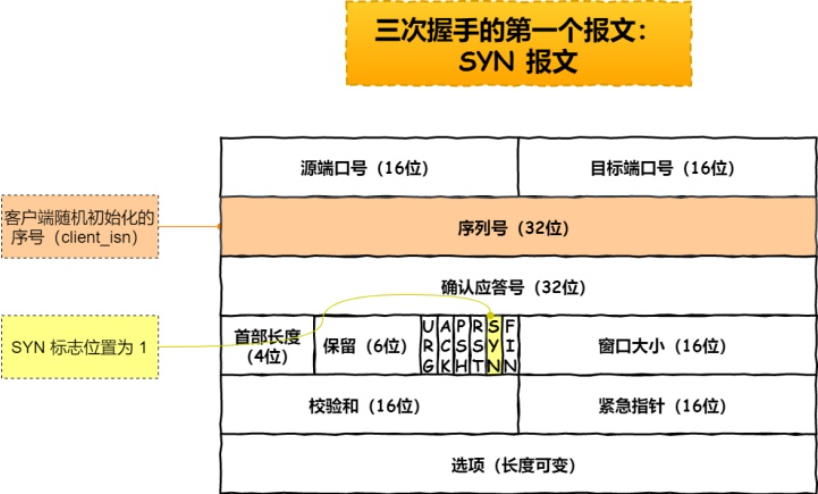
\includegraphics[width=.8\linewidth]{a4.png}
	\end{figure}

\item 客户端会随机初始化序号(client\_isn),将此序号置于 TCP 首部的「序号」字段中,同时把 SYN 标志位置为 1 ,表示 SYN 报文。接着把第一个 SYN 报文发送给服务端,表示向服务端发起连接,该报文不包含应用层数据,之后客户端处于 SYN-SENT 状态。
	\begin{figure}[H]
	\centering
	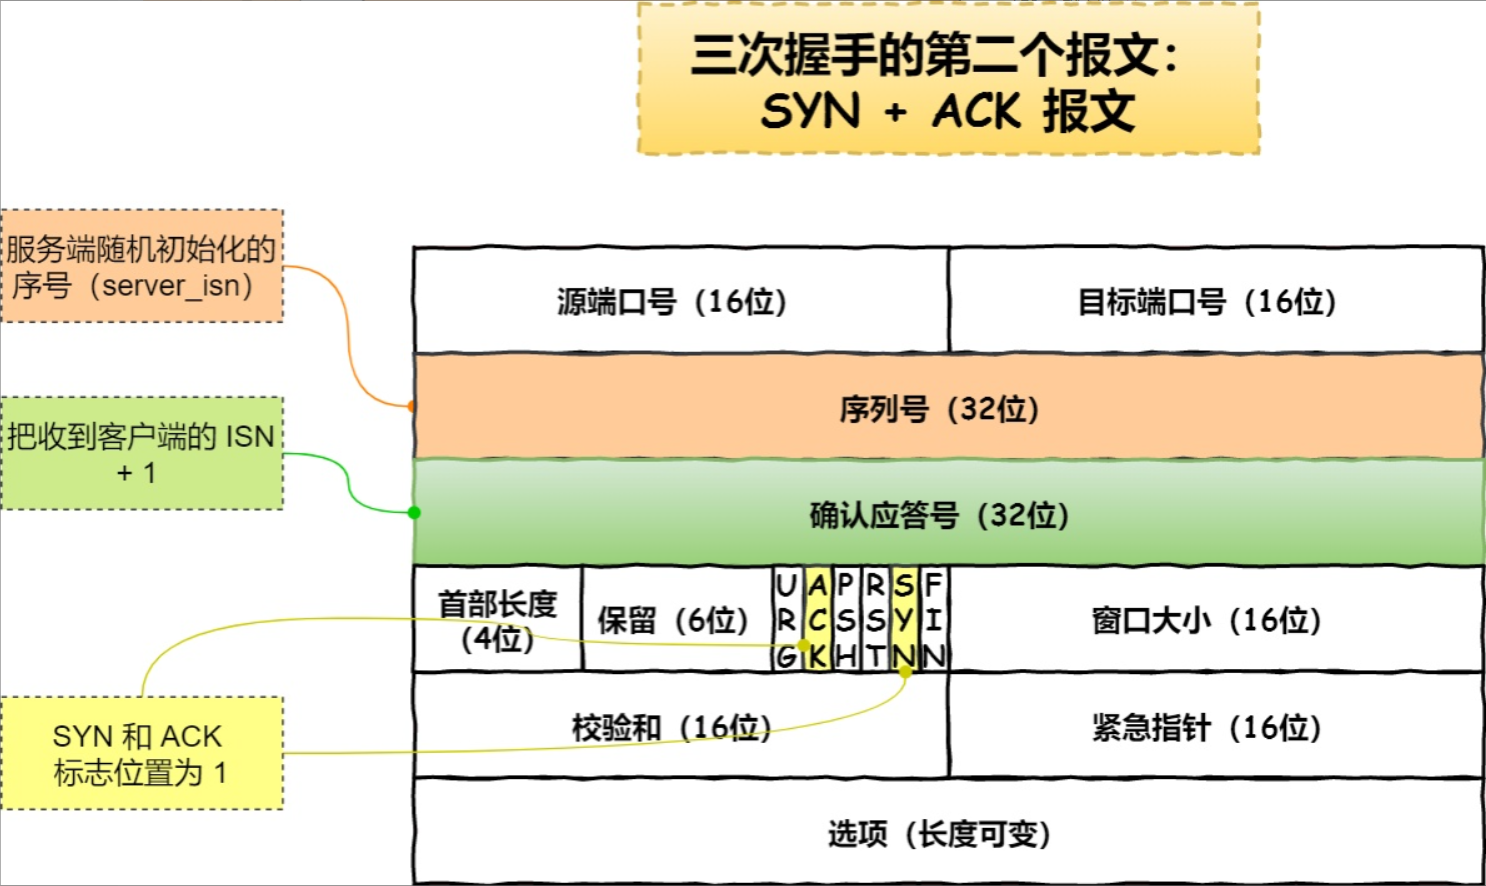
\includegraphics[width=.8\linewidth]{a5.png}
\end{figure}







\end{dinglist}






\chapter{笔记区}
\section{TCP/IP模型介绍}

\subsection{OSI七层模型}
七层模型,也称OSI(Open System Interconnection)参考模型。用于计算机或通信系统间互联的标准体系。一般称为OSI参考模型或七层模型。它从低到高分别是:物理层、数据链路层、网络层、传输层、会话层、表示层和应用层。
\begin{figure}[H]
	\centering
	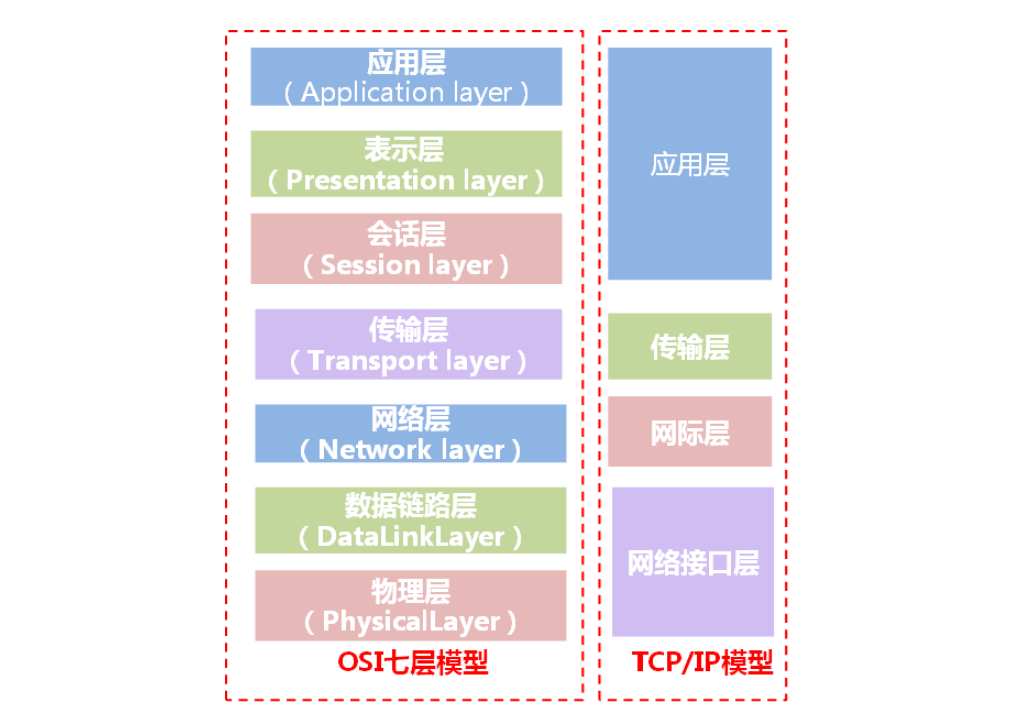
\includegraphics[width=\linewidth]{001.png}
\end{figure}
\begin{dinglist}{118}
	\item \textbf{应用层:}就是应用软件使用的协议,如邮箱使用的POP3,SMTP、远程登录使用的Telnet、获取IP地址的DHCP、域名解析的DNS、网页浏览的http协议等;这部分协议主要是规定应用软件如何去进行通信的。(应用层此部分有修改,感谢@小张指正。)
	
	 \item \textbf{表示层:}决定数据的展现(编码)形式,如同一部电影可以采样、量化、编码为RMVB、AVI,一张图片能够是JPEG、BMP、PNG等。
	 
	 \item \textbf{会话层:}为两端通信实体建立连接(会话),中间有认证鉴权以及检查点记录(供会话意外中断的时候可以继续,类似断点续传)。
	 
	 \item \textbf{传输层:}将一个数据/文件斩件分成很多小段,标记顺序以被对端接收后可以按顺序重组数据,另外标记该应用程序使用的端口号及提供QOS。(不同的应用程序使用不同计算机的端口号,同样的应用程序需要使用一样的端口号才能正常通信)
	 
	 \item \textbf{网络层}:路由选路,选择本次通信使用的协议(http、ftp等),指定路由策略及访问控制策略。(IP地址在这一层)
	 
	 \item \textbf{数据链路层:}根据端口与MAC地址,做分组(VLAN)隔离、端口安全、访问控制。(MAC地址在这一层)处理VLAN内的数据帧转发,跨VLAN间的访问,需要上升到网络层。
	 
	 \item \textbf{物理层:}将数据最终编码为用0、1标识的比特流,然后传输。(例如将题主头像的图片,变为一串01100111100这样的数字来表示)。
\end{dinglist}
\begin{warning}[title={{\color{green} \faEnvira} 为什么需要分层设计:\ }]
	如果没有分层设计,各个软件广商需要设计所有通信细节,包含物理层接口与信号编码,地址寻址,传输机制与保障。
	
	(腾讯做通信软件,Cisco做路由器 和交换机,安普做网线和水晶头)
\end{warning}




\begin{warning}[title={{\color{green} \faEnvira} OSI参考模型遵循的几大原则:\ }]
\begin{dinglist}{118}
	\item 各个层之间有\textbf{清晰的边界},便于理解;
	\item 每个层实现\textbf{特定的功能,且相互不影响;}
\begin{enumerate}
	\item 处理特定的应用程守细节
	\item 为两台主机上的麻用程序提供端到端的通讯
	\item 处理分组在服络中的活动,北例如分组选路
\end{enumerate}
	\item 每个层是\textbf{服务者又是被服务者,}热即为上午层服务, 又被下一层服务;
	\item 层次的划分有利于国际标佳协议的制定:
\begin{enumerate}
	\item IEEE负责数据链路层及其以下标准的指定
	\item IETE负责网络层及基以上标准的制肇
\end{enumerate}	
	
\item 层次的数目应该足够多, \textbf{以避免各个层功能重复。}
\end{dinglist}
\end{warning}


\begin{warning}[title={{\color{green} \faEnvira} OSI参考模型遵循的几大优点:\ }]
	\begin{dinglist}{118}
		\item 简化了相关的网络操作
		\item 提供即插即用的兼容性和不同咸商之间的标准接口
		
		思科的路由器, 可以接华为的交换机,可以跑腾讯的应用
		
		\item 使备个厂商能够设计出互操作的网络设备,加快数据通信网络发展,(两台路由器只要都采用标准的OSPF,是完全可以互相交换路由信息的)
		
		\item 防止一个区域网络的变化影响另一个区域的网络,因此,每一个区域的网络都能单独快速升级(IPv6)
		
		\item 把复杂的网络问题分解为小的简单问题(路由技术,交换技术,传输技术),易于学习和操作。
	\end{dinglist}
\end{warning}


\subsection{TCP/IP模型}
OSI 只是存在于概念和理论上的一种模型,它的缺点是分层太多,增加了网络工作的复杂性,所以没有大规模应用。后来人们对 OSI 进行了简化,合并了一些层,最终只保留了 4 层,从下到上分别是接口层、网络层、传输层和应用层,这就是大名鼎鼎的 TCP/IP 模型。

 TCP/IP五层协议和OSI的七层协议对应关系如下。
\begin{figure}[H]
	\centering
	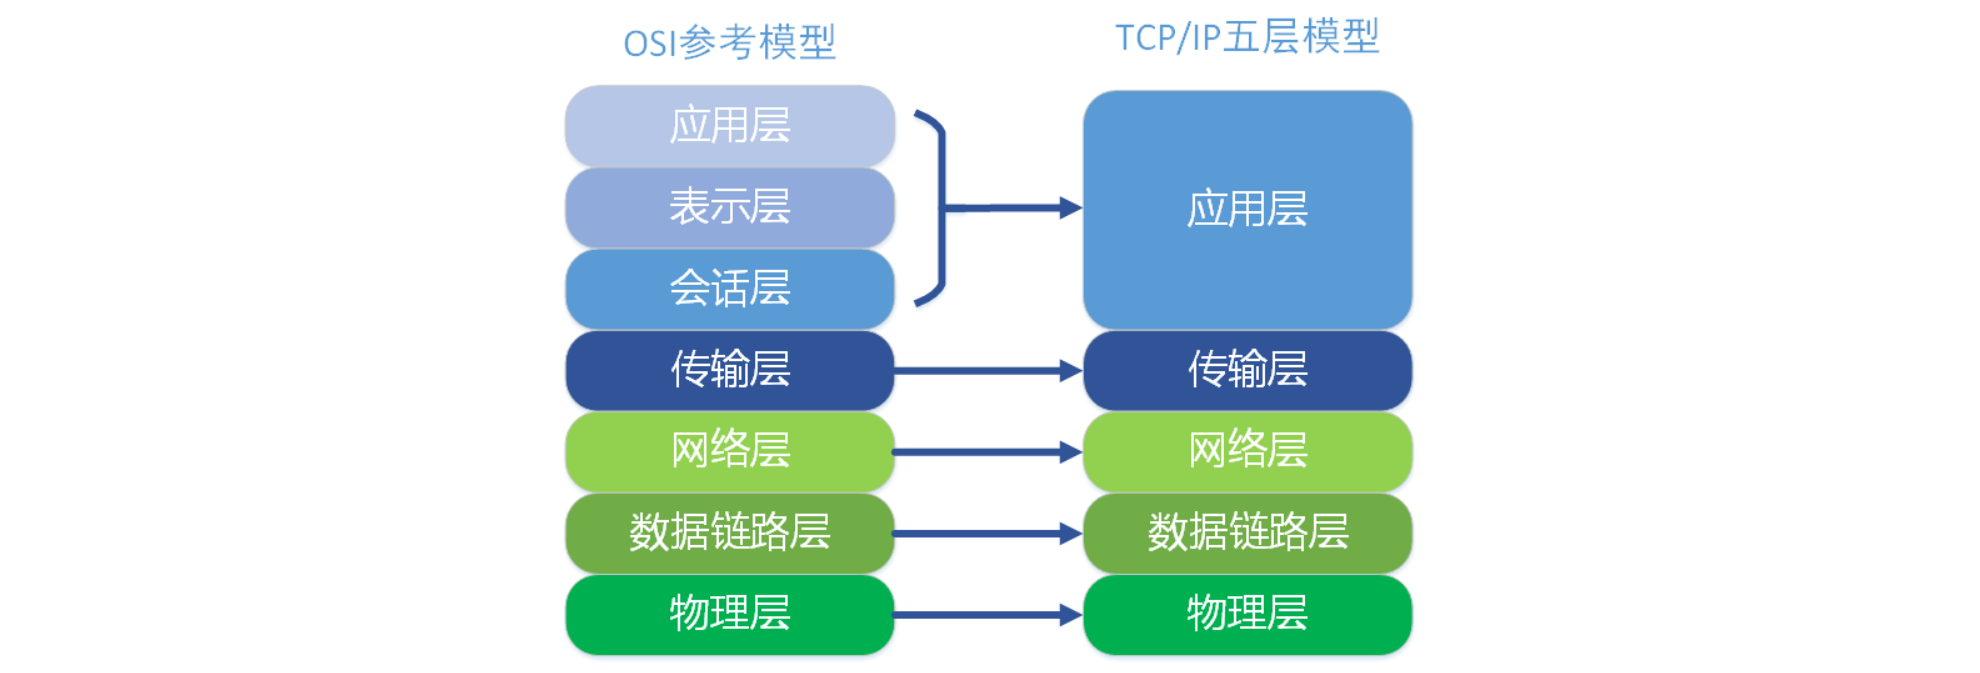
\includegraphics[width=\linewidth]{002.png}
\end{figure}

在每一层都工作着不同的设备,比如我们常用的交换机就工作在数据链路层的,一般的路由器是工作在网络层的。
\begin{figure}[H]
	\centering
	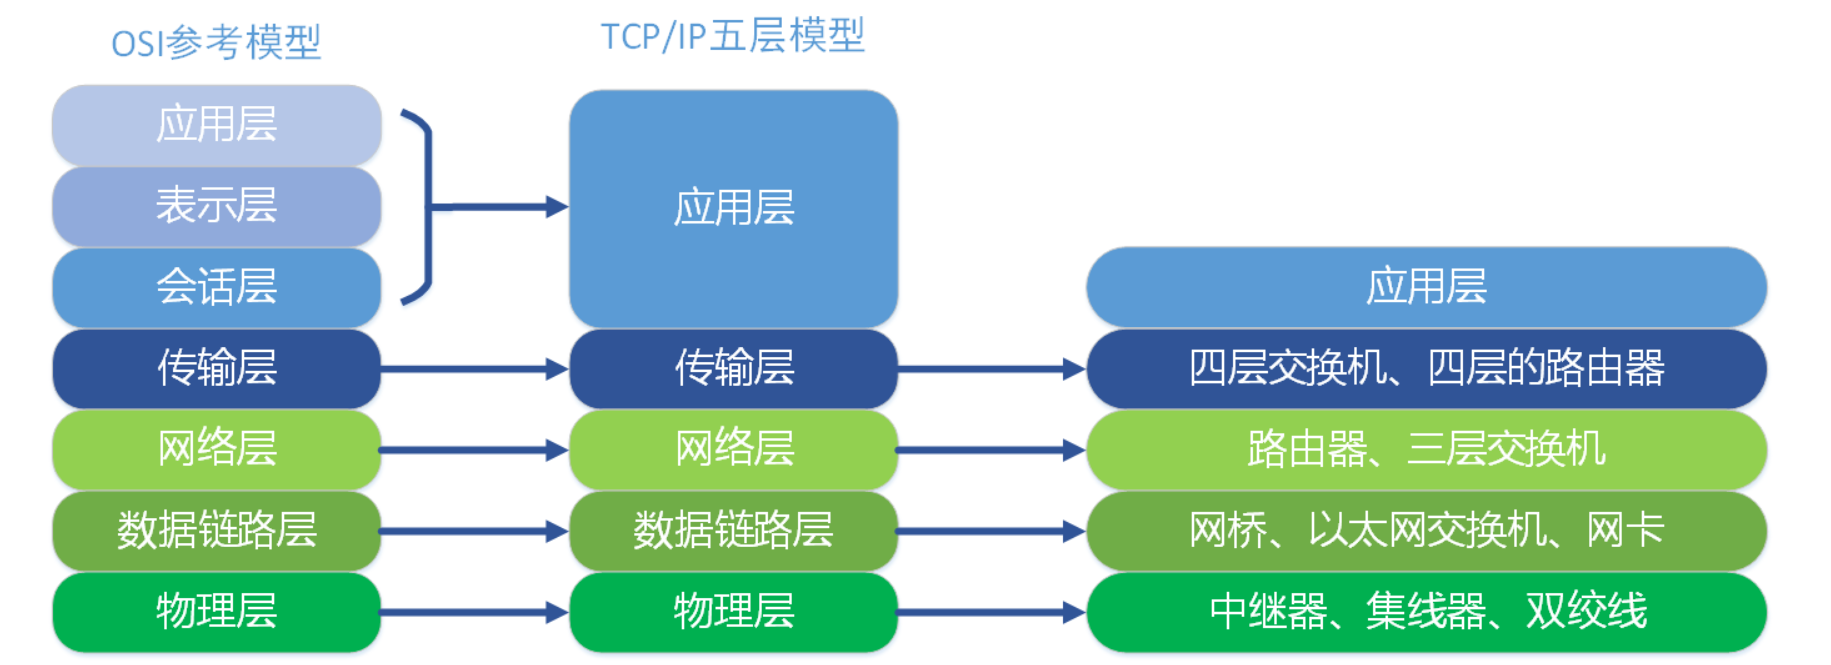
\includegraphics[width=\linewidth]{003.png}
\end{figure}
在每一层实现的协议也各不同,即每一层的服务也不同.下图列出了每层主要的协议。其中每层中具体的协议,我会在后面的逐一学习。
\begin{figure}[H]
	\centering
	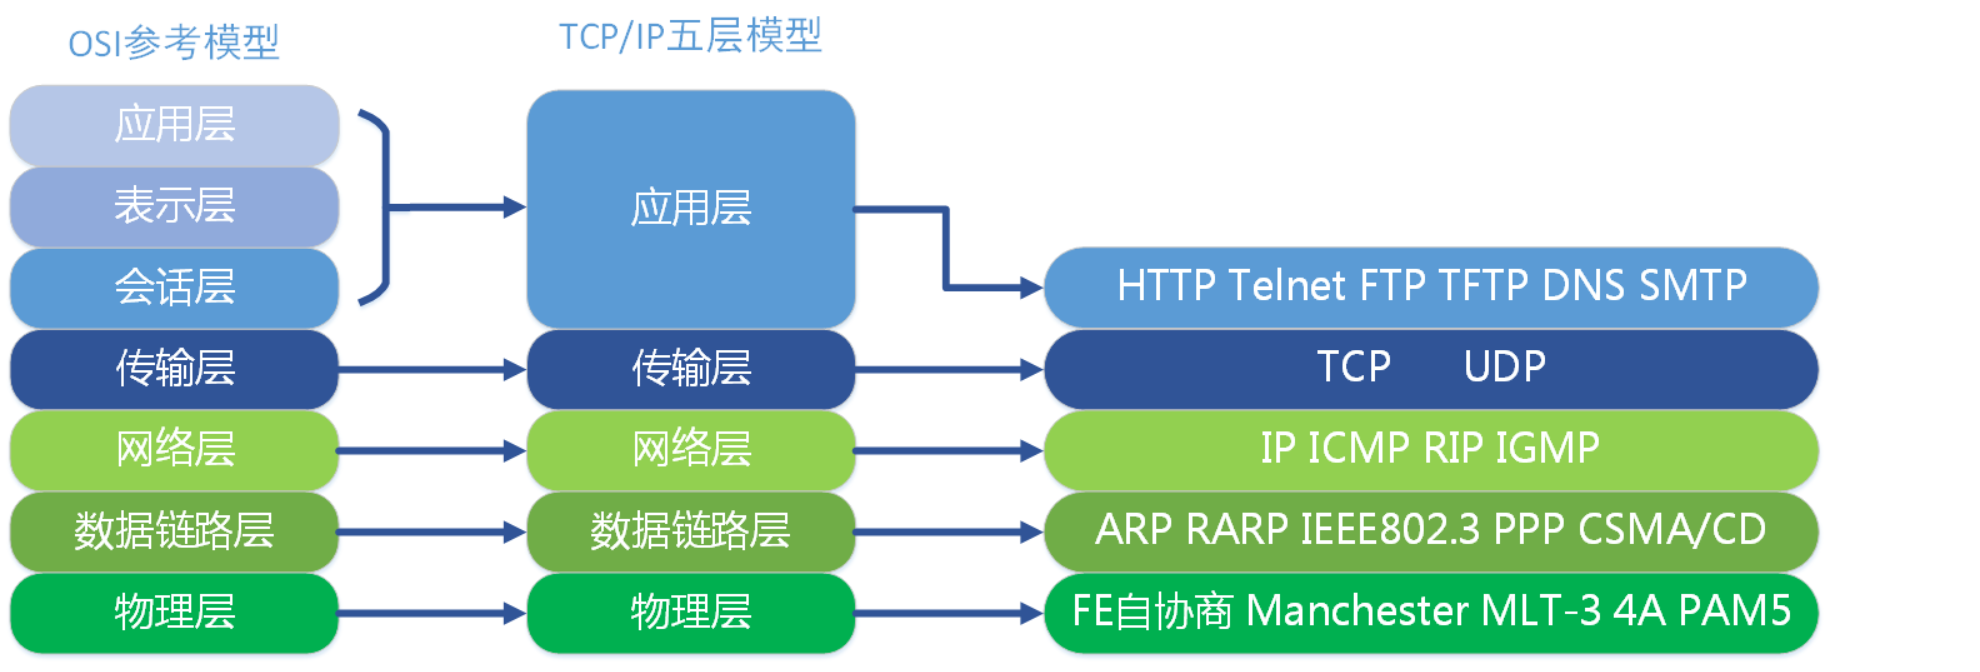
\includegraphics[width=\linewidth]{004.png}
\end{figure}

应用层:应用层确定进程之间通信的性质以满足用户的需要。

传输层:解决进程间的通信。

网络层:解决跨网络的主机通信问题。

数据链路层:解决相邻主机通信问题。

物理层:物理层的任务就是透明地传输比特流。



模型示意图
\begin{figure}[H]
	\centering
	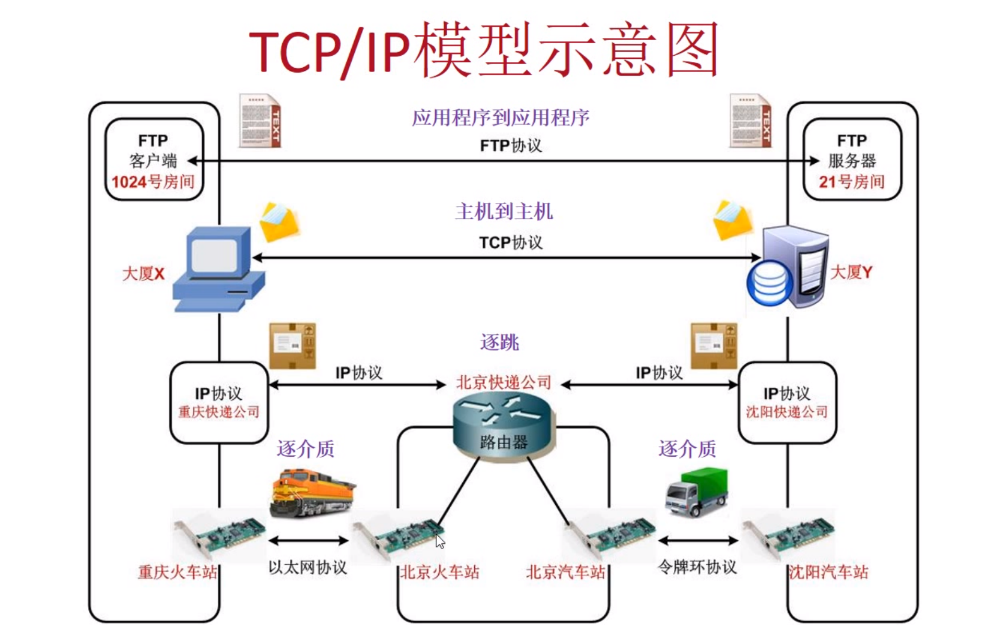
\includegraphics[width=\linewidth]{005.png}
\end{figure}

\begin{dinglist}{118}
	\item \textbf{应用层(FTP协议):}
	
	首先我们说说应用层,应用层就像在特定城市特定大厦特定房间内的某一个用户,应用层之间的通讯就像两个不同用户之间发送的信,这个信是点对点的,从一个用户(某一主机内特定应用程序)到另外一个特定用户(另一主机内特定应用程序)。一个主机(大厦)内可能有很多应用程序(客户),我们如何区分它们呢,实际生活中我们用房间号,在电脑内部区分不同应用程序我们用端口号。
	
	\item \textbf{传输层(TCP):}
	
	用户写好了信,需要给信套上信封,并且写好发件人所在大厦,和收件人所在大厦,实际生活中的大厦完全可以类比为我们的计算机和服务器。传输层(TCP)就是在两个不同主机之间传输信息的协议。
	
	\item\textbf{ 网络层(IP):}
	
	邮件准备好了,他首先会被送到本城市的快递公司,并且被打包,包裹上会写着源是重庆快递公司,目的是沈阳快递公司,但是重庆快递公司发现它不能直接发货到沈阳,需要通过北京快递公司进行中转。所以虽然目的是沈阳,但是他首先把这个包裹发给了北京。某个城市的快递公司就像IP协议,要抵达目的IP,需要查询路由表,如果发现目的地址不是直连就需要找下一跳。通过了解快递公司的工作,我们了解到IP协议是逐跳工作的。每一跳(路由器)根据目的IP地址查询下一跳,并且最终转发到目的地。
	
	\item \textbf{链路层(以太网):}
	
	重庆快递公司已经知道他需要把包裹发给北京快递公司了,现在他就把包裹送到重庆火车站,搭上去往北京的火车,然后在北京火车站卸货。然后送到北京快递公司,北京快递公司再判断下一跳为沈阳快递公司,并且选择适当的传输方式,例如:汽车,最后通过这种传输方式送到目的地沈阳快递公司。链路层协议就像包裹的运输方式,我们可以选择以太网(火车),也可以选择令牌环(汽车)。并且链路层协议是逐介质的,从一个网卡(重庆火车站)到另外一个网卡(北京火车站)。
	所以你会发现一个数据包从源到目的,IP地址总是不变的(源是重庆快递公司,目的是沈阳快递公司),但是链路层协议却在不断变化,第一跳源是重庆火车站,目的是北京火车站,第二跳源是北京汽车站,目的是沈阳汽车站。
\end{dinglist}



\begin{figure}[H]
	\centering
	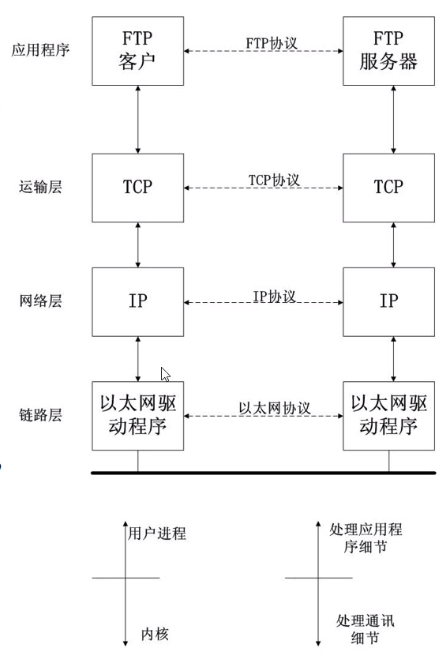
\includegraphics[width=.5\linewidth]{006.png}
\end{figure}
\section{以太网协议介绍}


\section{IP协议介绍}


\section{UDP协议介绍}


\section{TCP协议介绍}


\section{Web协议介绍}
\begin{warning}[title={{\color{green} \faEnvira} 完成一个用户输入注册:\ }]
1. 用于输入自己的用户名

2. 用户输入合法性检测

3. 写入数据库(写入文件)
\end{warning}
实现方法如下:
\begin{code}
	\vspace{-10pt}
	\begin{lstlisting}[style=Python2]
import json

def interactive():
	name = input('>>').strip()
	pwd = input('>>').strip()
	return {
		'name': name,
		'pwd': pwd
		}

def check(user_info):
	is_valid = True
	if len(user_info['name']) == 0:
		print('用户名为空')
		is_valid = False
	if len(user_info['pwd']) < 6:
		print('密码不能小于6位')
		is_valid = False
	return {
		'is_valid': is_valid,
		'user_info': user_info
		}

def register(check_info):
	if check_info['is_valid']:
		with open('db.json', 'w', encoding='utf-8') as f:
			json.dump(check_info['user_info'], f)

def main():
	user_info = interactive()
	check_info = check(user_info)
	register(check_info)

if __name__ == '__main__':
	main()
	\end{lstlisting}
	\vspace{-10pt}
\end{code}

\textbf{现在需要在上述过程中,添加邮箱验证功能}


\section{笔记区}
网络层:一个IP到一个IP的传输

传输层:一个应用到一个应用


应用层和传输层使用: end-to-end(端到端协议)

网络层使用:网络层提供的是逐跳(hop-to-hop)协议 

网络IP提供的是一种不可靠的服务, 他只是尽可能快的把分组从源结点送 到目的结点,但不提供可靠性保障。 

\textbf{TCP在不可靠的IP层上提供一个可靠的运输层} 

互联网的目的之一就是在应用程序中隐藏所有的物理细节


\subsection{可靠的TCP与不可靠的IP }
\begin{figure}[H]
	\centering
	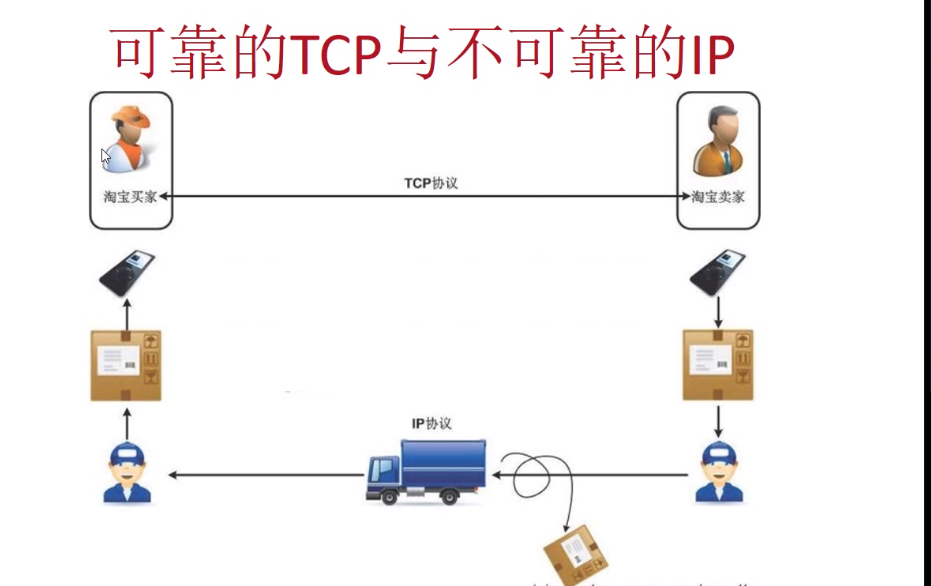
\includegraphics[width=\linewidth]{008.png}
\end{figure}
我们可以把淘宝买卖双方的关系,比作可靠的传输层TCP,因为他们之间的交易是需要确认的是可靠的。如果买家没有收到货物,肯定不能给卖家确认。但是快递公司可比作不可靠的网络层协议(IP)。卖家把一部销售给买家的手机封在一个包裹内(IP封包的过程),并且把这个包裹交给快递。对于快递的收件员,其实他并不清楚这个包裹内的东西是什么,他只用负责把这个包裹按照上面写的地址送到买家的手中(IP路由的过程)。由于网络层协议(IP)和快递一样不总是都靠谱,所以丢包是难免的。一旦出现丢包,长期没有收到快递的愤怒的买家就会找到卖家,倒霉的卖家只能把那部手机重新再发一次(一般快递都会推脱责任不予赔偿),这个过程就叫做TCP的超时重传。流着泪的卖家把新的包裹再次交给收件员,对于卖家而言这确实是再次。但是对于收件员而言,这只是一个普通的包裹,绝对不可能知道这是上次丢失包裹的一次重传。(这也是网络分层的目的,向下层隐藏上层的工作细节)。非常幸运的是,这次快递公司“不辱使命”成功完成了任务,把包裹交给了淘宝买家,买家对手机进行检查并且给卖家进行确认(TCP对数据的确认),本次会话结束。

\begin{figure}[H]
	\centering
	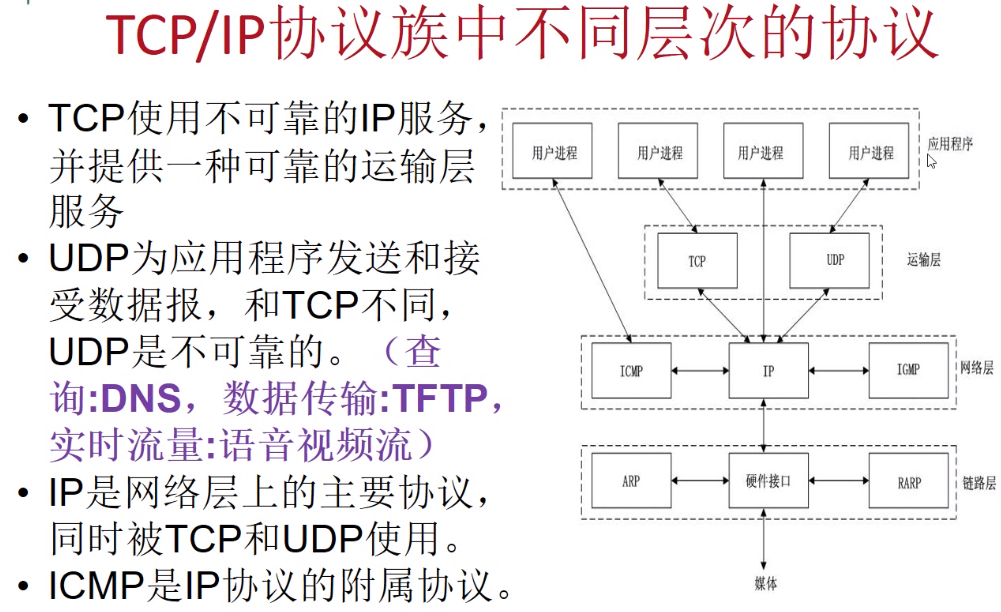
\includegraphics[width=\linewidth]{0081.png}
\end{figure}
・TCP使用不可靠的IP服务, 并提供一种可靠的运输层服务 

UDP为应用程序发送和接收数据报,和TCP不同,
UDP是不可靠的。\textbf{(查 询:DNS,数据传输:TFTP, 实时流量:语音视频流)} 

IP是网络层上的主要协议, 同时被TCP和UDP使用

ICMP是IP协议的附属协议


\begin{figure}[H]
	\centering
	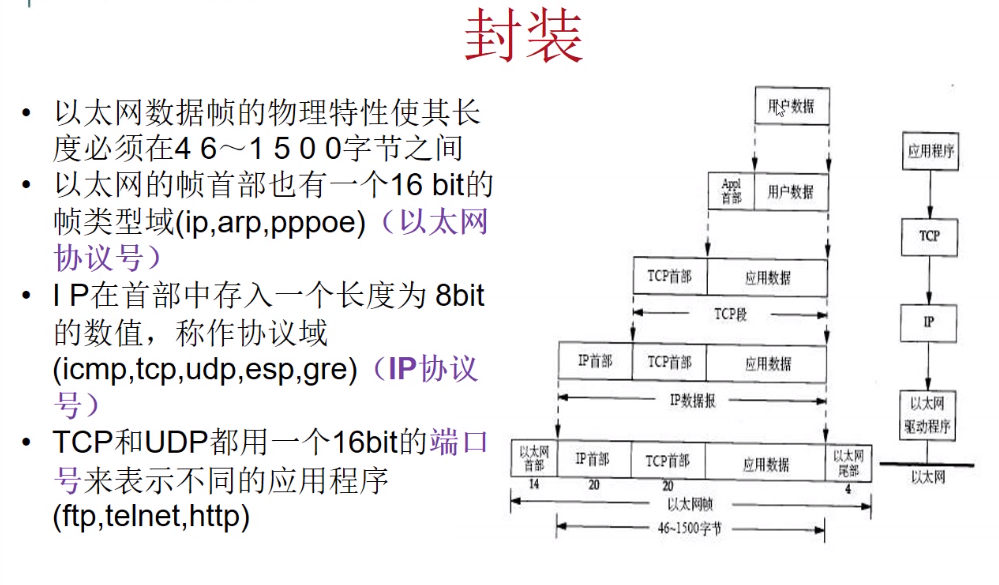
\includegraphics[width=\linewidth]{0091.png}
\end{figure}
\end{document}
